\documentclass[crop,tikz,convert={outext=.svg,command=\unexpanded{pdf2svg \infile\space\outfile}},multi=false]{standalone}

\usepackage{amsmath}
\usepackage{amssymb}
\usepackage{mathtools}
\usepackage{fullpage}
\usepackage[T1]{fontenc}
\usepackage{lmodern}
\usepackage{tikz}
\usetikzlibrary{calc,intersections,through,backgrounds}
\usetikzlibrary{bayesnet}
\usepackage{tikzscale}
\usepackage{tkz-euclide}
\usepackage{tcolorbox}
\tcbuselibrary{skins,breakable}
% pgfplots
\usepackage{pgfplots}
\pgfplotsset{compat=1.8}
% For entities in text
\newcommand{\entity}[1]{\texttt{#1}}
% For entities in pgfplots
\newcommand{\entpgf}[1]{\texttt{#1}}

\begin{document}
	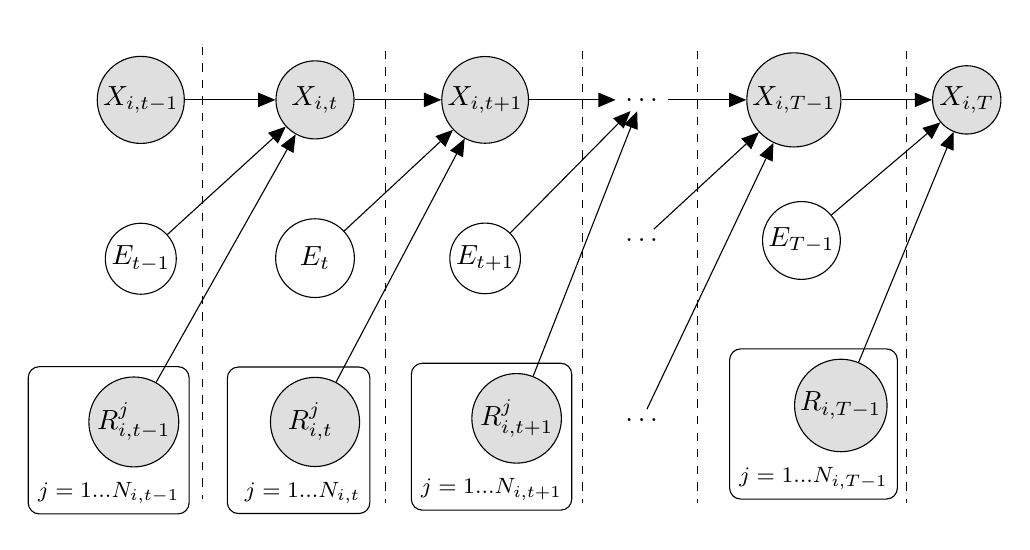
\begin{tikzpicture} %
		% Time t
		%\node[latent] (It) {$~I_{i,t}~$} ; %
		\node[obs] (Xt) {$~X_{i,t}~$} ; %
		\node[latent, below=of Xt,minimum width=1cm] (Et) {$~E_t~$} ;
		\node[obs, below=of Et] (Rt) {$~R_{i,t~}^j~$} ; %
		\plate {} {(Rt)} {$~j = 1...N_{i,t}$} ;
		%\node[obs, above=of Rt] (Mt) {$~M_{i,t}~$} ;
		%\node[above=of Rt] (Mt) {} ;
		%%%%% Time t-1
		\node[obs, left=of Rt,xshift=-0.15cm] (Rtm1) {$R_{i,t-1}^j$} ; %
		\plate {} {(Rtm1)} {$j = 1...N_{i,t-1}$} ;
		%\node[latent, left=of It] (Itm1) {$I_{i,t-1}$} ;
		\node[obs, left=of Xt,xshift=-0.15cm] (Xtm1) {$X_{i,t-1}$} ;
		%\node[obs, above=of Rtm1] (Mtm1) {$M_{i,t-1}$} ; %
		%\node[above=of Rtm1] (Mtm1) {} ;
		\node[latent, below=of Xtm1] (Etm1) {$E_{t-1}$} ;
		%%%%% Time t+1
		%\node[latent, right=of It] (Itp1) {$I_{i,t+1}$} ;
		\node[obs, right=of Xt,xshift=0.1cm] (Xtp1) {$X_{i,t+1}$} ;
		\node[latent, below=of Xtp1] (Etp1) {$E_{t+1}$} ;
		\node[obs, below=of Etp1, xshift=0.4cm, yshift=0.0cm] (Rtp1) {$R_{i,t+1}^j$} ;
		\plate {} {(Rtp1)} {$j = 1...N_{i,t+1}$} ;
		%%%%% dots
		\node[right=of Xtp1,xshift=0.1cm] (Xdots) {$\ldots$} ;
		\node[below=of Xdots,yshift=-0.5cm] (Edots) {$\ldots$} ;
		\node[below=of Edots,yshift=-1cm] (Rdots) {$\ldots$} ;
		%%%%% T-1
		\node[obs, right=of Xdots] (XTm1) {$X_{i,T-1}$} ;
		\node[latent, right=of Edots, xshift=0.2cm] (ETm1) {$E_{T-1}$} ;
		\node[obs, below=of ETm1, xshift=0.5cm, yshift=0.0cm] (RTm1) {$R_{i,T-1}$} ;
		\plate {} {(RTm1)} {$j = 1...N_{i,T-1}$} ;
		%%%%% T
		\node[obs, right=of XTm1,xshift=0.15cm] (XT) {$X_{i,T}$} ;
		% For dotted lines
		% t-1 to t
		\node[left=of Xt, xshift=0.2cm, yshift=0.8cm] (D1) {} ;
		\node[below=of D1, yshift=-4.74cm] (D2) {} ;
		% t to t+1
		\node[left=of Xtp1, xshift=0.42cm, yshift=0.75cm] (D3) {} ;
		\node[below=of D3, yshift=-4.74cm] (D4) {} ;
		% t+1 to dots
		\node[left=of Xdots, xshift=0.7cm, yshift=0.75cm] (D5) {} ;
		\node[below=of D5, yshift=-4.74cm] (D6) {} ;
		% dots to T-1
		\node[left=of XTm1, xshift=0.5cm, yshift=0.75cm] (D7) {} ;
		\node[below=of D7, yshift=-4.74cm] (D8) {} ;
		% T-1 to T
		\node[left=of XT, xshift=0.8cm, yshift=0.75cm] (D9) {} ;
		\node[below=of D9, yshift=-4.74cm] (D10) {} ;
		% Time t
		%\edge {It} {Mt} ;
		\edge {Xtm1} {Xt} ;
		\edge {Xt} {Xtp1} ;
		\edge {Etm1} {Xt} ;
		\edge {Et} {Xtp1} ;
		\edge {Rtm1} {Xt} ;
		\edge {Rt} {Xtp1} ;
		\edge {Xtp1} {Xdots} ;
		\edge {Xdots} {XTm1} ;
		\edge {Etp1} {Xdots} ;
		\edge {Rtp1} {Xdots} ;
		\edge {Edots} {XTm1} ;
		\edge {Rdots} {XTm1} ;
		\edge {XTm1} {XT} ;
		\edge {ETm1} {XT} ;
		\edge {RTm1} {XT} ;
		% Time t+1
		% Dotted
		\edge [-, dashed] {D1} {D2} ;
		\edge [-, dashed] {D3} {D4} ;
		\edge [-, dashed] {D5} {D6} ;
		\edge [-, dashed] {D7} {D8} ;
		\edge [-, dashed] {D9} {D10} ;
	\end{tikzpicture}
	%\caption{The basic model of intellectual influence used to interpret diachronic shifts in the word embedding spaces generated throughout the study, where each $X_{i,t}$ node represents an observed texts published by author $i$ at time $t$, each $E_t$ node represents the collection of historically-salient non-textual events which occurred at time $t$, each $R_{i,t}$ node represents a particular text read by author $i$ at time $t$ (the superscript $j$ indexing among multiple texts read within the same time period), and successive time periods are separated by dashed vertical lines.}
	%\label{fig:pgm-influence}
\end{document}
